\documentclass[tikz,border=8pt]{standalone}
\usepackage{tikz}
\usepackage{amsmath}
\usepackage{xcolor}
\usetikzlibrary{shapes.geometric}
\begin{document}
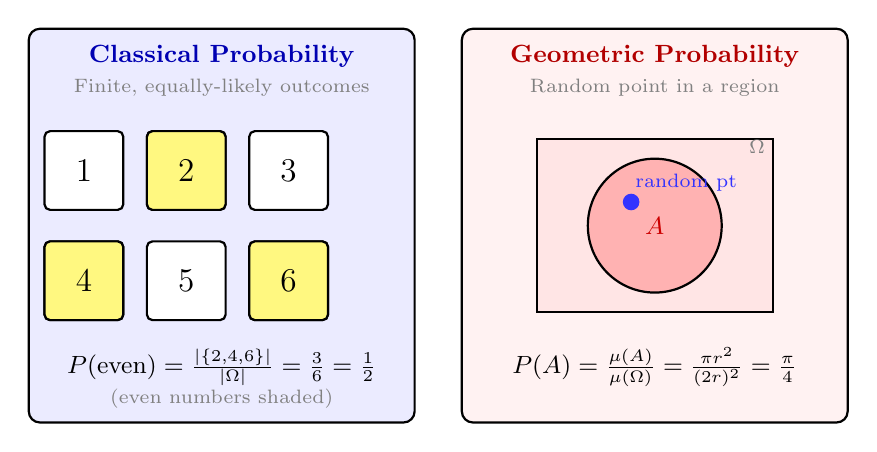
\begin{tikzpicture}[scale=1.0]

  %% ---- Left panel: Classical probability (dice) ----
  \draw[thick,rounded corners=4pt,fill=blue!8] (-5.2,-2.5) rectangle (-0.3,2.5);
  \node[font=\bfseries\small,blue!70!black] at (-2.75,2.15) {Classical Probability};
  \node[font=\scriptsize,gray] at (-2.75,1.75) {Finite, equally-likely outcomes};

  % Draw 6 dice faces in a 2x3 grid
  \foreach \col/\val in {1/1, 2/2, 3/3} {
    \draw[thick,rounded corners=2pt,fill=white]
      ({-5.0+(\col-1)*1.3}, 0.2) rectangle ({-5.0+(\col-1)*1.3+1.0}, 1.2);
    \node[font=\large] at ({-5.0+(\col-1)*1.3+0.5}, 0.7) {\val};
  }
  \foreach \col/\val in {1/4, 2/5, 3/6} {
    \draw[thick,rounded corners=2pt,fill=white]
      ({-5.0+(\col-1)*1.3}, -1.2) rectangle ({-5.0+(\col-1)*1.3+1.0}, -0.2);
    \node[font=\large] at ({-5.0+(\col-1)*1.3+0.5}, -0.7) {\val};
  }

  % Highlight even numbers
  \foreach \col in {2} {
    \draw[thick,rounded corners=2pt,fill=yellow!50]
      ({-5.0+(\col-1)*1.3}, 0.2) rectangle ({-5.0+(\col-1)*1.3+1.0}, 1.2);
    \node[font=\large] at ({-5.0+(\col-1)*1.3+0.5}, 0.7) {2};
  }
  \foreach \col/\val in {1/4, 3/6} {
    \draw[thick,rounded corners=2pt,fill=yellow!50]
      ({-5.0+(\col-1)*1.3}, -1.2) rectangle ({-5.0+(\col-1)*1.3+1.0}, -0.2);
    \node[font=\large] at ({-5.0+(\col-1)*1.3+0.5}, -0.7) {\val};
  }

  % Formula
  \node[font=\small] at (-2.75,-1.8) {$P(\text{even}) = \frac{|\{2,4,6\}|}{|\Omega|} = \frac{3}{6} = \frac{1}{2}$};
  \node[font=\scriptsize,gray] at (-2.75,-2.2) {(even numbers shaded)};

  %% ---- Right panel: Geometric probability (disk) ----
  \draw[thick,rounded corners=4pt,fill=red!5] (0.3,-2.5) rectangle (5.2,2.5);
  \node[font=\bfseries\small,red!70!black] at (2.75,2.15) {Geometric Probability};
  \node[font=\scriptsize,gray] at (2.75,1.75) {Random point in a region};

  % Outer square (sample space)
  \draw[thick,fill=red!10] (1.25,-1.1) rectangle (4.25,1.1);
  \node[font=\scriptsize,gray] at (4.05,1.0) {$\Omega$};

  % Inner circle (event A)
  \draw[thick,fill=red!30] (2.75,0) circle (0.85);
  \node[font=\small,red!80!black] at (2.75,0) {$A$};

  % Random dot
  \fill[blue!80] (2.45,0.3) circle (3pt);
  \node[font=\scriptsize,blue!80] at (3.15,0.55) {random pt};

  % Formula
  \node[font=\small] at (2.75,-1.8) {$P(A) = \frac{\mu(A)}{\mu(\Omega)} = \frac{\pi r^2}{(2r)^2} = \frac{\pi}{4}$};

\end{tikzpicture}
\end{document}
